\usepackage{xcolor}
\usepackage{afterpage}
\usepackage{pifont,mdframed}
\usepackage[bottom]{footmisc}


\createsection{\Grader}{Sample Grader}
\createsection{\Specs}{Clarifications}

\renewcommand{\inputfile}{\texttt{stdin}}
\renewcommand{\outputfile}{\texttt{stdout}}
\makeatletter
\renewcommand{\this@inputfilename}{\texttt{stdin}}
\renewcommand{\this@outputfilename}{\texttt{stdout}}
\makeatother

\newenvironment{warning}
  {\par\begin{mdframed}[linewidth=2pt,linecolor=gray]%
    \begin{list}{}{\leftmargin=1cm
                   \labelwidth=\leftmargin}\item[\Large\ding{43}]}
  {\end{list}\end{mdframed}\par}

\newenvironment{todoenv}
{\par\begin{mdframed}[linewidth=2pt,linecolor=red]%
		\begin{list}{}{\leftmargin=1cm
				\labelwidth=\leftmargin}\item[\Large\ding{169}]}
		{\end{list}\end{mdframed}\par}

\newcommand{\todo}[1]{\begin{todoenv}
		TODO: #1
\end{todoenv}}

% % % % % % % % % % % % % % % % % % % % % % % % % % % % % % % % % % % % % % % % % % %
% % % % % % % % % % % % % % % % % % % % % % % % % % % % % % % % % % % % % % % % % % %


As OII tradition wants, the contest day precedes the long celebrations night. The organizers will throw a wild party in full Trentino style, during which boys and girls will party hard. Obviously, for ``partying hard'' we mean to indulge in intellectually stimulating activities which, at the same time, aren't too tiring!

This year, the selected activity was: building an incredibly long chain of dominoes.

\begin{wrapfigure}[10]{r}{0.4\textwidth}
  \vspace{-30pt}
  \begin{center}
    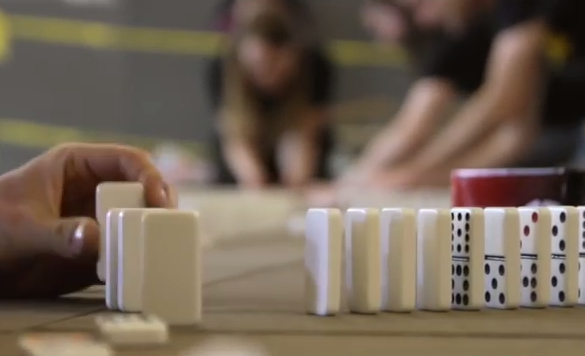
\includegraphics[width=0.9\linewidth]{domino.png}
    \caption{Athletes at work}
  \end{center}
\end{wrapfigure}

The party lasts all night and is abruptly interrupted when Monica
comes to take the athletes to the famous Galilei gymnasium, where the awards ceremony will take place.

 
So far, athletes have been able to place in $N$ tiles, each one
exactly $1$ centimeter away from the previous one.

Not having enough traditional tiles, they used whatever they could get a hold of:
each ``tile'' could therefore be a few centimeters high but also
several meters!

Athletes now want to conclude the party
in great style, by pushing the first card and crashing the whole domino chain.

The fall of a tile of height $h$ causes the fall of the following $h-1$ tiles:
so a tile of height $1$ doesn't cause the fall of any other tile.

Because of the exhaustion of the long night, the athletes fear that they might have misplaced
some tile.


There is no time to rebuild everything: help them understand if it's possible to swap two tiles (but only two!) so that the whole domino chain will fall!

\begin{mdframed}[backgroundcolor=black!10,rightline=false,leftline=false]

\Specs

\small

The tiles are indexed from $0$ to $N-1$.
Position $0$ is the leftmost and the tiles fall from left to right.

After making the exchange, the card in position $0$ is dropped first.

If the card at index $i$ falls, and its height is $h$, then all the cards in the positions up to $i+h-1$ (included) will fall.

The tile in position $0$ always drops, and a tile in position $i \geq 1$
falls if and only if there is a card in position $i' < i$ that falls, with height of at least $i-i'+1$.

Note that all tiles fall if and only if the tile in position $N-1$ falls.

\end{mdframed}

\pagebreak

% % % % % % % % % % % % % % % % % % % % % % % % % % % % % % % % % % % % % % % % % % %
% % % % % % % % % % % % % % % % % % % % % % % % % % % % % % % % % % % % % % % % % % %

\Implementation


You will need to submit a single file with extension \texttt{.cpp} or \texttt{.c}.

\begin{warning}
Attached to this task you will find a template \texttt{catena.cpp} and \texttt{catena.c}
with an implementation example.
\end{warning}

You will need to implement the following function.

\begin{center}\begin{tabularx}{\textwidth}{|c|X|}
\hline
C/C++  & \verb|stato_t correggi(int N, int altezze[], coppia_t* scambio);|\\
\hline
\end{tabularx}\end{center}

\begin{itemize}[nolistsep]
  \item The integer number $N$ represents the number of tiles.
  \item
    The \texttt{altezze} array, indexed from $0$ to $N-1$, contains the height of each tile.
    The tile is initially in position $i$, for $0 \leq i \leq N-1$, has height $\texttt{altezze}[i]$.
  \item
    The data type \texttt{stato\_t} is an \texttt{enum} that can assume values
    \texttt{OK}, \texttt{SOLVED} or \texttt{IMPOSSIBILE}.
    The function must return:
    \begin{itemize}
      \item \texttt{OK}, if no swap is required for all the tiles to fall; otherwise,
      \item \texttt{SOLVED},
        if it is possible to swap two tiles
        so that, after that, all the tiles fall; otherwise,
      \item \texttt{IMPOSSIBILE},
        when a single exchange is not enough.
    \end{itemize}
  \item
    The data type \texttt{coppia\_t} is a \texttt{struct} which contains the fields
    \texttt{domino1} and \texttt{domino2}.
    If the function returns \texttt{SOLVED},
    the fields \texttt{domino1} and \texttt{domino2}
    of the output parameter \texttt{scambio}
    must be populated with the positions of the two tiles to be swapped.
\end{itemize}

The function \texttt{correggi} will be called only once.
The return value of the function will be recorded and,
if this value is \texttt{SOLVED},
the positions in the \texttt{scambio} struct will be stored as well.

% % % % % % % % % % % % % % % % % % % % % % % % % % % % % % % % % % % % % % % % % % %
% % % % % % % % % % % % % % % % % % % % % % % % % % % % % % % % % % % % % % % % % % %


\Grader
You can find a simplified version of the grader used during the competition in this task's directory. You can use it to test your solutions. The sample grader reads data from \inputfile{}, calls the functions that you have to implement and writes on \outputfile{}, according to the following format.

The input file consists of $2$ rows, containing:
\begin{itemize}[nolistsep,itemsep=2mm]
\item row $1$, integer number $N$;
\item row $2$, integer numbers \texttt{heights[$i$]}, for $i = 0\ldots N-1$, separated by spaces.
\end{itemize}

The output file consists of a single line that contains one of the following options:
\begin{itemize}[nolistsep,itemsep=2mm]
\item the string \texttt{OK}, if the domino chain is completely knocked down without any swap;
\item the string \texttt{IMPOSSIBLE}, if it is not possible to adjust the chain with only one swap;
\item two integer numbers $i$ and $j$, separated by space,
  if you can adjust the chain by swapping the tiles in the positions $i$ and $j$.
\end{itemize}

% % % % % % % % % % % % % % % % % % % % % % % % % % % % % % % % % % % % % % % % % % %
% % % % % % % % % % % % % % % % % % % % % % % % % % % % % % % % % % % % % % % % % % %

\pagebreak
\Constraints

\begin{itemize}[nolistsep, itemsep=2mm]
	\item $1 \le N \le 5\,000\,000$.
	\item $1 \le \texttt{altezze}[i] \le 1000$ for each $i=0, \ldots, N-1$.
\end{itemize}

% % % % % % % % % % % % % % % % % % % % % % % % % % % % % % % % % % % % % % % % % % %
% % % % % % % % % % % % % % % % % % % % % % % % % % % % % % % % % % % % % % % % % % %


\Scoring

Your program will be tested on several test cases grouped into subtasks.
To get the score for a subtasks, you must correctly solve all the tests in it.

\begin{itemize}[nolistsep,itemsep=2mm]
  \item \textbf{\makebox[2cm][l]{Subtask 1} [\phantom{0}0 punti]}: Sample cases.
  \item \textbf{\makebox[2cm][l]{Subtask 2} [\phantom{0}4 punti]}: The heights are all the same.
  \item \textbf{\makebox[2cm][l]{Subtask 3} [\phantom{0}7 punti]}: $N \le 5000$, the answer is \texttt{OK} or \texttt{IMPOSSIBILE}.
  \item \textbf{\makebox[2cm][l]{Subtask 4} [\phantom{0}9 punti]}: The answer is \texttt{OK} or \texttt{IMPOSSIBILE}.
  \item \textbf{\makebox[2cm][l]{Subtask 5} [13 punti]}: $N \leq 50$.
  \item \textbf{\makebox[2cm][l]{Subtask 6} [19 punti]}: $N \leq 1000$.
  \item \textbf{\makebox[2cm][l]{Subtask 7} [28 punti]}: $N \leq 3000$.
  \item \textbf{\makebox[2cm][l]{Subtask 8} [11 punti]}: $N \leq 100\,000$.
  \item \textbf{\makebox[2cm][l]{Subtask 9} [\phantom{0}9 punti]}: No specific limitations.
\end{itemize}

% % % % % % % % % % % % % % % % % % % % % % % % % % % % % % % % % % % % % % % % % % %
% % % % % % % % % % % % % % % % % % % % % % % % % % % % % % % % % % % % % % % % % % %


\Examples

\begin{example}
\exmpfile{caduta.input0.txt}{caduta.output0.txt}%
\exmpfile{caduta.input1.txt}{caduta.output1.txt}%
\exmpfile{caduta.input2.txt}{caduta.output2.txt}%
\end{example}

% % % % % % % % % % % % % % % % % % % % % % % % % % % % % % % % % % % % % % % % % % %
% % % % % % % % % % % % % % % % % % % % % % % % % % % % % % % % % % % % % % % % % % %

\pagebreak
\Explanation

In \textbf{first example} it's sufficient to exchange the tiles in positions $2$ and $3$:

\begin{center}
	\includegraphics[scale = 1.5]{asy_caduta/fig1.pdf}
\end{center}

In \textbf{second example} the tile at position $2$ is high enough: the chain is fine as it is.

\begin{center}
	\includegraphics[scale = 1.5]{asy_caduta/fig2.pdf}
\end{center}

In \textbf{third example} the tiles are too low: it's impossible for the chain to fall.

\begin{center}
	\includegraphics[scale = 1.5]{asy_caduta/fig3.pdf}
\end{center}
